\begin{figure}
  \centering
  \usetikzlibrary{shapes.arrows, fadings}
  \definecolor{LightColor}{rgb}{1.0,0.901,0.805}

  \definecolor{tile0}{HTML}{DABDE4}
  \definecolor{tile1}{HTML}{B8DBF4}
  \definecolor{tile2}{HTML}{B5EDCD}
  \definecolor{tile3}{HTML}{FBEBA7}
  \definecolor{tile4}{HTML}{F9C1BB}

  \tikzstyle{array_element}=[rectangle,
                             minimum height=1cm, 
                             minimum width=1cm, 
                             minimum size=1cm,
                             draw=black,
                             rounded corners=2.5, ]
  \tikzstyle{grid_element}=[rectangle,
                            minimum height=1.5cm, 
                            minimum width=1.5cm, 
                            draw=black,
                            rounded corners=2.5, ]
  \tikzstyle{grid_element_big}=[rectangle, 
                               minimum height=2cm, 
                               minimum width=2cm, 
                               draw=black,
                               rounded corners=2.5, ]

  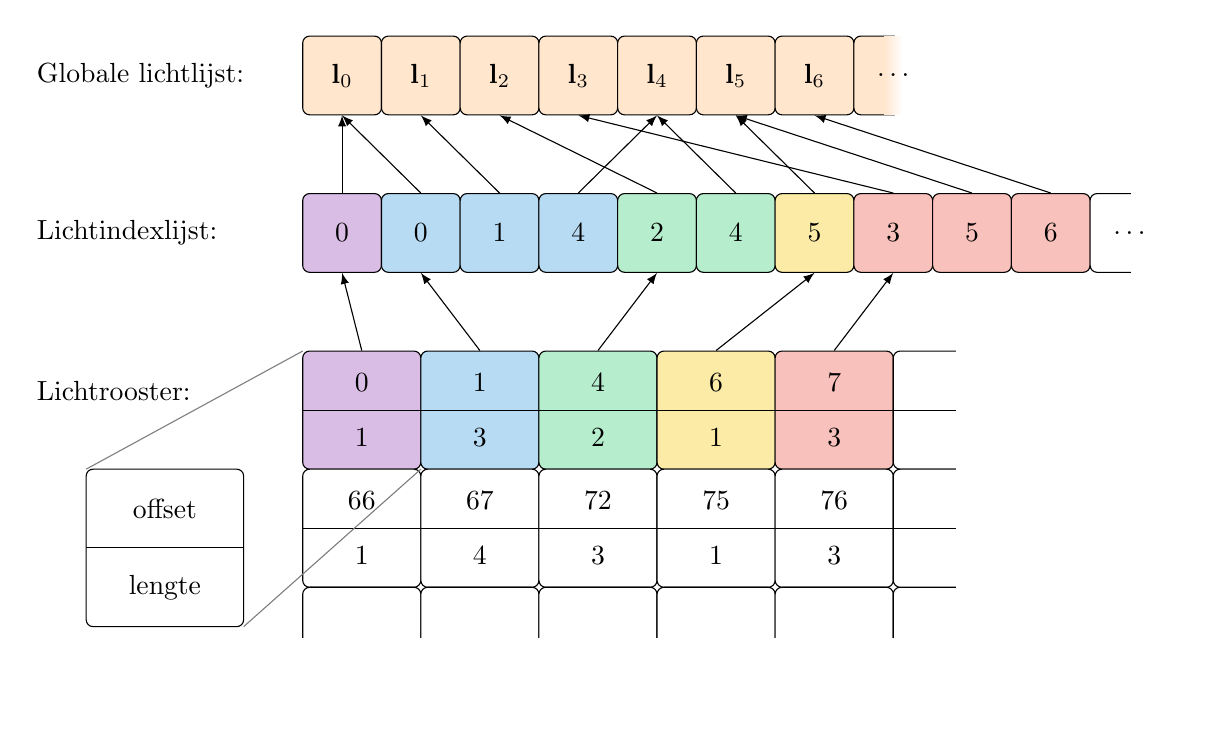
\begin{tikzpicture}
    \node at (-4.cm, 4cm) (light_list_name) [anchor=west] {Globale lichtlijst:};
    \node at (-4.cm, 2cm) (light_list_name) [anchor=west] {Lichtindexlijst:};
    \node at (-4.cm, 0cm) (light_list_name) [anchor=west] {Lichtrooster:};

    \foreach \l in {0,...,6} {
      \node at (1cm * \l, 4cm) (light_\l) [array_element,fill={LightColor}] {$\mathbf{l}_\l$};
    }
    \node at (1cm * 7, 4cm) [array_element, fill={LightColor}, ] {};
    \node at (1cm * 7.325, 4cm) [rectangle,
                                 minimum height=1.2cm,
                                 minimum width=0.6cm,
                                 fill={white},
                                 draw=white] {};
    \node at (1cm * 7, 4cm) [rectangle,                    
                             minimum height=0.98cm, 
                             minimum width=0.2cm, 
                             shading = axis,
                             shading angle=90,
                             left color=LightColor ] {};
                                         
    \node at (1cm * 7, 4cm) [rectangle, minimum height=1cm, minimum width=1cm] {$\dots$};

    \foreach \i/\l in {0/0} {
      \node at (1cm * \i, 2cm) (light_index_\i) [array_element, fill={tile0}] {\l};
      \draw[-latex] (light_index_\i.north) -- (light_\l.south);
    }
    \foreach \i/\l in {1/0, 2/1, 3/4} {
      \node at (1cm * \i, 2cm) (light_index_\i) [array_element, fill={tile1}] {\l};
      \draw[-latex] (light_index_\i.north) -- (light_\l.south);
    }
    \foreach \i/\l in {4/2, 5/4} {
      \node at (1cm * \i, 2cm) (light_index_\i) [array_element, fill={tile2}] {\l};
      \draw[-latex] (light_index_\i.north) -- (light_\l.south);
    }
    \foreach \i/\l in {6/5} {
      \node at (1cm * \i, 2cm) (light_index_\i) [array_element, fill={tile3}] {\l};
      \draw[-latex] (light_index_\i.north) -- (light_\l.south);
    }
    \foreach \i/\l in {7/3, 8/5, 9/6} {
      \node at (1cm * \i, 2cm) (light_index_\i) [array_element, fill={tile4}] {\l};
      \draw[-latex] (light_index_\i.north) -- (light_\l.south);
    }
    \node at (1cm * 10, 2cm) [array_element,
                              fill={white}, ] {};
    \node at (1cm * 10.325, 2cm) [rectangle,
                                  minimum height=1.2cm,
                                  minimum width=0.6cm,
                                  fill={white},
                                  draw=white] {};
    \node at (1cm * 10, 2cm) [rectangle,
                              minimum height=1cm,
                              minimum width=1cm] {$\dots$};

    \foreach \i/\off/\len/\p in {0/0/1/0, 
                                 1/1/3/0, 
                                 2/4/2/0, 
                                 3/6/1/0, 
                                 4/7/3/0 } {
      \node at (0.25cm + 1.5cm * \i, -0.25cm) (grid_\i) [grid_element, fill={tile\i}] {};
      \node at (-0.625cm + 1.5cm * \i , -0.25cm) (grid_l) [] {};
      \node at (1.125cm + 1.5cm * \i, -0.25cm) (grid_r) [] {};
      \draw (grid_l) -- (grid_r);
      \node at (0.25cm+ 1.5cm * \i, 0.1cm) [] { \off };
      \node at (0.25cm+ 1.5cm * \i, -0.6cm) [] { \len };
    }
    \foreach \i/\off/\len in {0/66/1,
                              1/67/4,
                              2/72/3,
                              3/75/1,
                              4/76/3 } {
      \node at (0.25cm + 1.5cm * \i, -1.75cm) [grid_element, fill={white}] {};
      \node at (-0.625cm + 1.5cm * \i , -1.75cm) (grid_l) [] {};
      \node at (1.125cm + 1.5cm * \i, -1.75cm) (grid_r) [] {};
      \draw (grid_l) -- (grid_r);
      \node at (0.25cm+ 1.5cm * \i, -1.4cm) [] { \off };
      \node at (0.25cm+ 1.5cm * \i, -2.1cm) [] { \len };
    }
    \foreach \i/\off/\len in {0/66/1, 1/67/4, 2/72/3, 3/75/1,4/76/3,5/0/0 } {
      \node at (0.25cm + 1.5cm * \i, -3.25cm) [grid_element, fill={white}] {};
    }
    \node at (0.25cm + 1.5cm * 5, -0.25cm) [grid_element, fill={white}] {};
    \node at (-0.625cm + 1.5cm * 5 , -0.25cm) (grid_l) [] {};
    \node at (1.125cm + 1.5cm * 5, -0.25cm) (grid_r) [] {};
    \draw (grid_l) -- (grid_r);

    \node at (0.25cm + 1.5cm * 5, -1.75cm) [grid_element, fill={white}] {};
    \node at (-0.625cm + 1.5cm * 5 , -1.75cm) (grid_l) [] {};
    \node at (1.125cm + 1.5cm * 5, -1.75cm) (grid_r) [] {};
    \draw (grid_l) -- (grid_r);

    \node at (4cm, -3.6cm) [rectangle, minimum height=0.9cm, minimum width=9.1cm, fill={white}] {};
    \node at (0.75cm + 5 * 1.5cm, -1.6cm) [rectangle, minimum height=4.5cm, minimum width=0.9cm, fill={white}] {};

    \draw[-latex] (grid_0.north) -- (light_index_0.south);
    \draw[-latex] (grid_1.north) -- (light_index_1.south);
    \draw[-latex] (grid_2.north) -- (light_index_4.south);
    \draw[-latex] (grid_3.north) -- (light_index_6.south);
    \draw[-latex] (grid_4.north) -- (light_index_7.south);

    \node at (-2.25cm, -2cm) (node_big) [grid_element_big] {};
    \node at (-3.25cm , -2cm) (grid_l) [] {};
    \node at (-1.25cm, -2cm) (grid_r) [] {};
    \draw (grid_l.center) -- (grid_r.center);
    \node at (-2.25cm, -1.5cm) [] { offset };
    \node at (-2.25cm, -2.5cm) [] { lengte };

    \node at (-3.25, -1cm) (node_big_up) [] {};
    \node at (-1.25, -3cm) (node_big_low) [] {};

    \node at (-0.5, 0.5cm) (node_small_up) [] {};
    \node at (1.0, -1cm) (node_small_low) [] {};

    \draw[gray] (node_big_up.center) -- (node_small_up.center);
    \draw[gray] (node_big_low.center) -- (node_small_low.center);
  \end{tikzpicture}
  \caption{De datstructuren van Tiled Shading.}
  \label{fig:ts-datastructuur}
\end{figure}
